\label{timing-chapter}

To demonstrate the extensibility of our methodology, we
decided to add a new, useful feature to mCertiKOS-secure:
the ability for user processes to time their own executions.
Timing flows pose a notoriously difficult challenge for
security reasoning. Nevertheless, we were able to successfully
implement and verify the security of this new feature with
only about two person-weeks of effort. The generality of the
observation function is extremely helpful for clearly specifying
how user processes view time.

%%%%%%%%%%%%%%%%%%%%%%%%%%%%%%%%%%%%%%%%%%%%%%%%%%%%%%%%%%%%%%%%
\begin{figure}[t]
\begin{center}
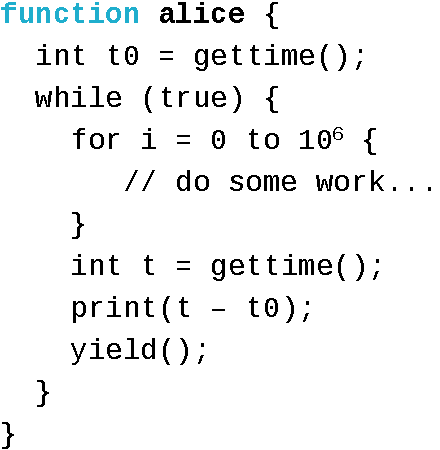
\includegraphics[scale=0.55]{pldi/figure/gettime}
\caption{\small A sample usage of the \gett{} feature.}
\label{fig:gettime}
%\vspace*{-20pt}
\end{center}
\end{figure}
%%%%%%%%%%%%%%%%%%%%%%%%%%%%%%%%%%%%%%%%%%%%%%%%%%%%%%%%%%%%%%%%

\section{Specification and Implementation of Timing}
Figure~\ref{fig:gettime} shows a motivating example for the
new feature that we would like to support. We wish to
provide a system call \gett{} that user processes
can invoke to help time their executions. However, we do
not want to allow processes to communicate with each other
by exploiting this timestamp. Hence we must create some notion
of \emph{virtualized} time, whereby each process has its
own isolated timeline.
It is important to note that the feature we are implementing
here is completely orthogonal to a wall-clock time. While
a user can observe the time of an event within the context of
his own timeline, our threat model still assumes that he has
no mechanism for associating that event with a global
wall-clock time.

\paragraph{TSC Oracle}
As a basis for implementing the timing feature, we make use of 
x86's Time Stamp Counter (TSC), which keeps track of the total
number of clock cycles since the last reset. At the machine model
level (MBoot), we add a new primitive \ttt{rd\_tsc}, and axiomatize
its specification. The primitive's implementation is unverified
but extremely simple: it looks up the current TSC value using
x86's RDTSC instruction, and returns the value. Note that the
TSC value clearly can be used as a potential information-flow
side channel; thus the \ttt{rd\_tsc} primitive is not exposed to
users at the TSysCall level, and users are not allowed to directly
invoke the RDTSC instruction (x86 has a global TSD flag which, 
when set, will cause a user-mode RDTSC invocation to trigger
an exception).

Defining the specification of \ttt{rd\_tsc} is somewhat subtle.
We certainly do not want to model the actual number of cycles on
the machine, since this is highly nondeterministic. A single
assembly instruction could take any number of cycles to
execute depending on various unpredictable conditions. Rather
than try to accurately specify the value of the TSC, we will instead assume 
the existence of an \emph{oracle} for a given execution that will 
accurately answer the question, ``for any $n$, what is the TSC 
value returned by the $n$th invocation of the RDTSC instruction?''
This strategy is reasonable because of the following two facts:
(1) our theorems will apply to \emph{any} choice of oracle; and 
(2) for every actual execution, there exists some oracle consistent 
with that execution.

%%%%%%%%%%%%%%%%%%%%%%%%%%%%%%%%%%%%%%%%%%%%%%%%%%%%%%%%%%%%%%%%
\begin{figure}[t]
\begin{center}
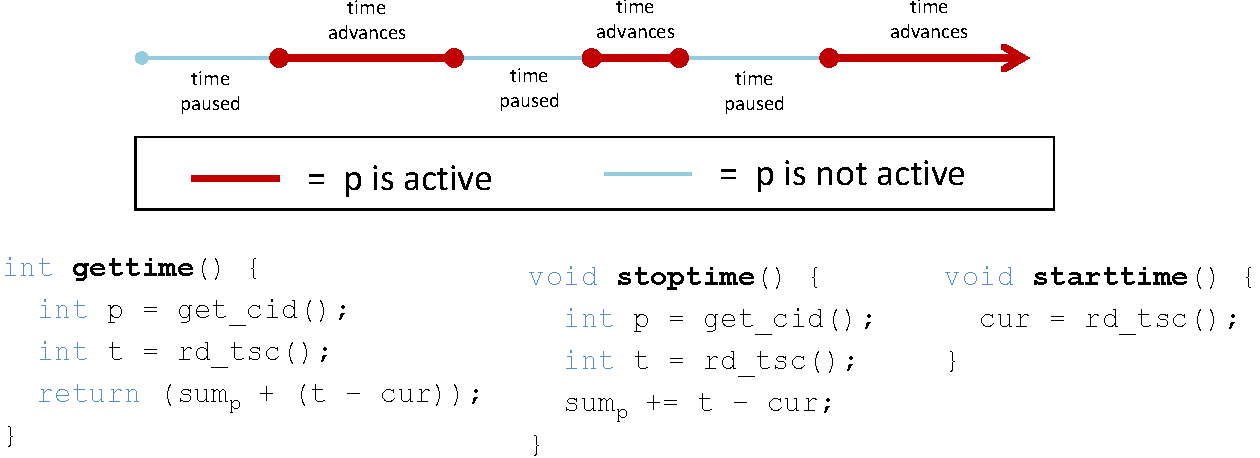
\includegraphics[scale=0.685]{pldi/figure/timeline}
\caption{\small Illustration and implementation of local timelines.}
\label{fig:timeline}
%\vspace*{-20pt}
\end{center}
\end{figure}
%%%%%%%%%%%%%%%%%%%%%%%%%%%%%%%%%%%%%%%%%%%%%%%%%%%%%%%%%%%%%%%%

\paragraph{Local Timeline}
Given our specification of the physical TSC in terms of an oracle,
we virtualize the TSC value for each user process by implementing
isolated timelines. Figure~\ref{fig:timeline} illustrates a
timeline that is local to process $p$, and shows the code that
implements all timelines. It is useful to think of our
implementation in terms of stopwatches. Each process has its
own stopwatch: \gett{} returns the value of the active
(i.e., currently-running) process's stopwatch, \stopt{}
pauses the active process's stopwatch, and \startt{} resumes
the active process's stopwatch. Whenever a process yields,
\stopt{} is called prior to context switching, the active 
process ID is changed to be
the head of the ready queue, and finally \startt{} is called after context 
switching. This
guarantees that, at any given moment during execution, all 
process's stopwatches are paused except for the active one.

The code of Figure~\ref{fig:timeline} shows a straightforward
way to implement these stopwatches. In the following, we will
use the term \emph{epoch} to refer to a portion of execution
in between two consecutive yields. We say that an epoch belongs
to process $p$ if $p$ is the active process during that epoch.
At any moment during an execution, we use the term 
\emph{current epoch} to refer to the portion of execution since
the most recent yield. Given this terminology, the stopwatch 
implementation uses the following two fields of program state:
\begin{itemize}
\item $\ttt{sum}_i$~--- For each process $i$, this integer value 
gives the total amount of time spent in previous completed epochs
belonging to $i$.
\item \ttt{cur}~--- This integer value records the TSC value of the
beginning of the current epoch.
\end{itemize}
Given these fields, the current virtualized time at any moment
can be computed as $\ttt{sum}_p + (t - \ttt{cur})$, where $p$ is the
active process and $t$ is the current TSC value returned by \ttt{rd\_tsc}. 
Whenever a yield occurs, the appropriate \ttt{sum} is 
increased by the length of the just-completed epoch (\ttt{stoptime}), and 
then \ttt{cur} is reset to the current TSC value (\ttt{starttime}). In this 
way, each process has its own virtualized timeline.

\paragraph{Aside on TSC Overflow}
Technically, we need to be concerned with errors in our code arising
from the TSC value overflowing. However, the TSC is a 64-bit value 
in x86 architecture, so a machine would have to be running for
well over a century on modern architecture in order for overflow
to occur. Therefore, we choose to embed an assumption within our
verification that the return value of \ttt{rd\_tsc} is always
less than $2^{64}$. Notice that this assumption implies that
the virtualized time $\ttt{sum}_p + (t - \ttt{cur})$
also does not overflow, since this value is a subset of the
timeline interval from 0 to $t$.

\section{Security of Virtualized Time}
The generality of the observation function allows for a clean and
simple security verification of virtualized time. For convenience,
we first add a field \ttt{tsc} to abstract state that represents 
the physical TSC. It gets updated to the return value of \ttt{rd\_tsc}
whenever that primitive is called. In other words, \ttt{tsc} simply
remembers the value that \ttt{rd\_tsc} returned the last time it 
was called. Given this, we define three timing-related observations made 
by process $p$:
\begin{itemize}
\item \emph{Previous Epochs}~--- The value of $\ttt{sum}_p$ is observable.
\item \emph{Current Epoch}~--- The value of ($\ttt{tsc} - \ttt{cur}$) is 
observable if $p$ is the active process.
\item \emph{Oracle}~--- The $p$-filtered subset of the TSC oracle is 
observable (discussion below).
\end{itemize}
The first two observations clearly imply that the virtualized time
$\ttt{sum}_p + (t - \ttt{cur})$ is always observable when
$p$ is the active process and $t$ is the value just returned by
\ttt{rd\_tsc}; this fact yields a simple security proof
of the \gett{} system call. Notice how we exploit generality of the
observation function here by making the difference between \ttt{tsc}
and \ttt{cur} observable, even though each of the two values individually
must be unobservable since they pinpoint timestamps on a \emph{global}
timeline rather than local.

%\noindent
The third observation is quite subtle. Consider the following 
two insights:
\begin{enumerate}
\item \emph{The oracle cannot be entirely unobservable.}
Recall that the specification of \gett{} first
sets $t$ to be the next value given by the oracle, and then 
returns $\ttt{sum}_p + (t - \ttt{cur})$. 
In order to prove that this specification is noninterfering,
we must know that the oracle produces the same $t$ value
in two indistinguishable states. Therefore the oracle cannot
be entirely hidden from observation.
\item \emph{The oracle cannot be entirely observable.} 
It is possible that in two executions
from indistinguishable states, a process $p'$ which is not the 
observer $p$ may invoke \gett{} a different number of times, implying
an information flow from $p'$ to $p$. In other words, the 
integrity lemma of Chapter~\ref{casestudy-proof-chapter} will
fail to hold if the entire oracle is observable to~$p$,
since other processes can clearly change the oracle by invoking
\gett{}.
\end{enumerate}
Together, these insights imply that only some portion of the
oracle can be observable to~$p$. In particular, we need to
somehow filter the oracle, observing only those entries
which correspond to \ttt{rd\_tsc} invocations made by $p$.
One potential solution would be to divide the single global
oracle into many per-process oracles. Unfortunately, this
solution makes it difficult to define the semantics of
\ttt{rd\_tsc} at the MBoot level. At the TSysCall level, we
would choose which oracle to query based on the currently-running
process, stored in the abstract data field \ttt{cid}; at the
MBoot level, however, \ttt{cid} has not yet been abstracted.
It might be possible to specify the MBoot-level semantics to
inspect the concrete memory corresponding to \ttt{cid}, but this
would cause all kinds of trouble since it would violate the mCertiKOS 
convention that primitive specifications never depend on concrete 
memory.

Instead, we use a simple solution that cleverly exploits our
assumption of safety of the high-level machine (the first
property of Definition~\ref{high-level-security} in 
Chapter~\ref{methodology-chapter}). For each natural
number $n$, we extend the oracle to return not only the
current TSC value, but also an integer $p$ representing a process
ID. At the TSysCall level, $p$ is used as a prerequisite for safe
execution: the specification of \gett{} checks whether $p$ is
equal to \ttt{cid}, and returns \none{} if this check fails.
At the MBoot level, on the other hand, $p$ is completely ignored
by the \ttt{rd\_tsc} specification, allowing us to define the
specification without a need to refer to \ttt{cid}. This means that there are
some oracles for which a TSysCall-level execution gets stuck, but
the corresponding MBoot-level execution is safe. Thankfully, this 
odd situation is irrelevant due to the fact that we assume safe
execution at the TSysCall level as a prerequisite for all of our
major theorems. Notice that
this solution is still justifiable in the following sense: even
though many choices of oracle will now yield faulty high-level 
execution, there still always exists some valid oracle for any 
actual, safe execution.

Given this extended definition of oracle, we can now 
$p$-filter an oracle by choosing only those entries with process
ID~$p$. Then, as mentioned above, we make only this $p$-filtered
oracle subset observable to~$p$. While the intuitive concept should
be clear at this point, the technical details of defining 
$p$-filtering are actually still a bit tricky. Because we represent
the oracle as a function from natural numbers to pairs, we also
keep track of the current natural-number position in abstract state.
Whenever \ttt{rd\_tsc} is called, this position is incremented
by one. When defining the observation, we must be careful how we
treat this oracle position, since it could be a source of information leak.
To make observability independent from the precise value of the oracle 
position, we define a function \ttt{filter}$(o,c,p,n)$ which takes oracle 
$o$, oracle position $c$, process ID $p$, and natural number $n$ as parameters, 
and returns the $n$th occurrence of pairs in $o$ with process ID equal
to $p$, starting from position $c$. Then oracle observation is defined 
as:
\[\observe{p}{\sigma} \isdef \lambda~n \such \ttt{filter}(\ttt{oracle}(\sigma),
\ttt{oracle\_pos}(\sigma),p,n)\]
In other words, rather than make the oracle position $c$ 
observable, we make the infinite stream of $p$-related
oracle entries starting from $c$ observable. 

With the help of a few simple lemmas characterizing this 
\ttt{filter} function, the entire security verification of virtualized 
time goes through quite easily. The generality of the observation
function is key in allowing us to prove security of this new kernel feature.
This clearly demonstrates the extensibility of our novel methodology: even 
though we need to introduce the concept of an oracle for reasoning about
time within mCertiKOS, the timing-sensitive security verification
is still completely straightforward.





